\chapter{Podwarstwa Radio Link Control}
\label{cha:rlc}

\begin{figure}
	\centerline{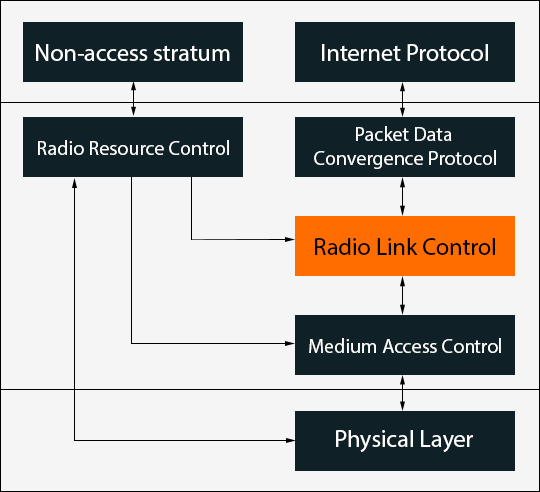
\includegraphics[width=0.4\textwidth]{images/rlc_overview.png}}
	\caption{Umiejscowienie podwarstwy RLC w stosie protokołów LTE}
	\label{fig:rlc_overview}
\end{figure}

Podwarstwa RLC (Radio Link Control) jest drugą z podwarstw warstwy Access Stratum. Odbiera ona jednostki danych z podwarstw PDCP oraz RRC a następnie przekazuje je do podwarstwy MAC. RLC może działać w jednym z 3 trybów transmisji: transparentnym, z potwierdzeniami lub bez potwierdzeń. Jest ona odpowiedzialna za:

\begin{enumerate}
	\item Segmentację i/lub łączenie transmitowanych jednostek danych
	\item Wykrywanie zduplikowanych jednostek danych podczas ich odbierania z niższych warstw
	\item Zapewnienie dostarczenia jednostek danych w odpowiedniej kolejności
	\item Naprawa błędów poprzez ponowne wysyłanie jednostek danych
\end{enumerate}

\section{Segmentacja i łączenie jednostek danych}
\label{sec:segmentation}

Zanim podwarstwa RLC po stronie urządzenia transmitującego prześle dane do odbiornika musi poczekać na informację z podwarstwy MAC o tym, że własnie pojawiła się możliwość transmisji danych. Do tego czasu podwarstwa RLC przechowuje jednostki danych, które otrzymała z wyższych warstw w buforze transmisyjnym (Transmission Buffer na Rys. \ref{fig:rlc_simulation}). Razem z informacją o możliwości transmisji podwarstwa MAC wysyła również informację o rozmiarze bloku transportowego czyli o tym jaka ilość danych może zostać przesłana. Rozmiar dostępnego bloku transportowego może być za każdym razem inny i zależy on m.in. od jakości połączenia. Z tego powodu podwarstwa RLC musi dostosowywać rozmiar jednostek danych wysyłanych do podwarstwy MAC do rozmiaru bloku transportowego.

W tym celu jednostki danych, zbyt duże aby w całości zmieścić się w bloku transportowym, są dzielone na mniejsze fragmenty i wysyłane w dwóch lub więcej blokach transportowych. Natomiast jeżeli jednostki danych są dużo mniejsze od bloku transportowego to kilka jednostek danych jest umieszczonych w pojedynczym bloku transportowym. Dzięki temu dostępna przepustowość jest wykorzystywana maksymalnie efektywnie. Po stronie odbiornika odebrane jednostki danych są umieszczane w buforze. Jeżeli możliwe jest z nich odtworzenie kompletnej jednostki danych wówczas są one łączone i wysyłane do wyższej warstwy.

Na Rys. \ref{fig:rlc_simulation} przedstawiono zrzut ekranu z wykonanej symulacji przedstawiający podwarstwę RLC. W centralnej części widoczny jest blok transportowy zawierający 3 jednostki SDU, które były na tyle małe aby razem, w całości zmieścić się w bloku transportowym.

\begin{figure}
	\centerline{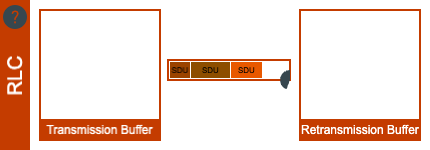
\includegraphics[width=0.5\textwidth]{images/rlc_transport_block.png}}
	\caption{Segmentacja SDU w bloku transportowym}
	\label{fig:rlc_simulation}
\end{figure}
  
\section{Wykrywanie zduplikowanych jednostek danych}

Błędy podczas transmisji danych mogą spowodować, że niektóre jednostki danych dotrą do odbiornika więcej niż raz. Warstwa RLC odpowiada za wykrycie zduplikowanych pakietów a następnie odrzucenie ich tak aby nie zostały ona przekazane do wyższych warstw. W tym celu każda jednostka danych podczas wysyłania posiada w nagłówku przypisany numer sekwencyjny. Z kolei odbiornik po swojej stronie utrzymuje bufor z odebranymi jednostkami danych. Jeżeli nowo odebrana jednostka danych posiada taki sam numer sekwencyjny jak jednostka danych która znajduje się w buforze oznacza to, że jest ona duplikatem i zostaje odrzucona.

\section{Zapewnienie kolejności}

Numer sekwencyjny, przypiswany do jednostek danych, jest również wykorzystywany do zapewnienia aby jednostki danych po stronie odbiornika były dostarczone przez podwarstwę RLC do wyższych warstw w tej samej kolejności w jakiej zostały one wysłane po stronie nadajnika. Oznacza to, że jednostka danych o numerze sekwencyjnym N musi zostać dostarczona przed jednostką danych o numerze sekwencyjnym N+1. Mechanizm ten działa w odmienny sposób dla trybu transmisji z potwierdzeniami i bez potwierdzeń dlatego też został dokładniej opisany w sekcjach \ref{subsec:um} i \ref{subsec:am}.

\section{Korekcja błędów}

O ile usługi typu VoIP mogą działać prawidłowo nawet jeżeli niewielka liczba pakietów nie dotrze od nadajnika do odbiornika to usługi typu HTTP lub FTP nie będa dziąłać prawidłowo jeżeli jakiekolwiek dane zostaną utracone. W tym celu podwarstwa RLC implementuje mechanizm ARQ (Automatic Repeat Request) który ma za zadanie wykrycie czy jakieś jednostki danych nie zostały dostarczone i zarządanie od nadawacy aby ponowił ich wysłanie. Mechanizm ten jest używany tylko w trybie transmisji z potwierdzeniami.

Po stronie odbiornika każda otrzymana jednostka danych jest weryfikowana pod kątem poprawności. W tym celu najczęściej używany jest mechanizm CRC (Cyclic Redundancy Check). Jeżeli odbiorca stwierdzi, że otrzymana jednostka danych jest błędna wysyła żądanie jej ponownej transmisji (NACK). Natomiast jednostka danych zostanie uznana za prawidłową zostaje wysłane potwierdzenie poprawnej transmisji (ACK). Po stronie nadawcy również dla każdej wysłanej jednostki danych startowany jest zegar, który odlicza czas do ponownej transmisji tej jednostki. Jeżeli przed upływem tego czasu zostanie otrzymane potwierdzenie (ACK) zegar jest zatrzymywana i jednostka danych usuwana z bufora po stronie nadawcy. W przeciwnym wypadku po upływie czasu jednostka danych jest ponownie transmitowana i odliczanie ponowione. Cały proces powtarza się dopóki nie zostanie odebrane potwierdzenie od odbiorcy lub dopóki cała komunikacja nie zostanie anulowana.


Wyróżnia się trzy typy mechanizmu ARQ:

\begin{enumerate}
	\item Stop-and-Wait ARQ - jest to najbardziej podstawowa forma mechanizmu ARQ. Nadawca wysyła jeden pakiet i oczekuje na potwierdzenie (ACK) lub żadanie ponownej transmisji (NACK) od odbiorcy a także startuje licznik czasowy. Jeżeli przed upływem czasu nie otrzyma potwierdzenia lub jeżeli otrzyma żadanie ponownej transmisji wówczas ponownie wysyła ten sam pakiet. Dopiero kiedy otrzyma od odbiorcy potwierdzenie (ACK) wówczas wysyła kolejny pakiet.
	\item Go-Back-N ARQ - w tym trybie określony jest pewien rozmiar okna transmisyjnego - N. Nadawca wysyła do N pakietów do odbiorcy a następnie oczekuje na ich potwierdzenia (ACK). Następnie sprawdza, które pakiety zostały potwierdzone i wznawia wysyłanie od pakietu o numerze sekwencyjnym, który jest kolejny po ostatnio potwierdzonym pakiecie. Odbiorca utrzymuje po swojej stronie informację o numerze sekwencyjnym następnego pakietu, który powinien dostać i ignoruje otrzymane pakiety jeżeli nie mają dokładnie tego numeru sekwencyjnego. Kiedy już otrzyma pakiet o wymaganym numerze sekwencyjnym wówczas wysyła do nadawcy potwierdzenie otrzymania pakietu (ACK) z załączonym numerem sekwencyjnym a następnie zwiększa u siebie oczekiwany numer sekwencyjny następnego pakietu o 1.
	\item Selective Repeat ARQ - w tym trybie również używane jest okno transmisyjne o danym rozmiarze - N. Nadawca wysyła N pakietów od odbiorcy. Odbiorca akceptuje kolejne pakiety, nawet jeżeli, któryś wcześniejszy pakiet był błędny lub nie dotarł. Odbiorca utrzymuje po swojej stronie najmniejszy numer sekwencyjny pakietu, który nie dotarł (lub był błędny) i wysyła go z każdym potwierdzeniem odebrania pakietów. Nadawca po wysłaniu N pakietów ponawia wysłanie pakietów, które nie dotarły do odbiorcy a następnie kontynuje wysyłanie pakietów od miejsca gdzie skończył.
\end{enumerate}

\section{Tryby transmisji}

\subsection{Transparentny}

Transparentny tryb transmisji jest używany przy przesyłaniu danych do kanałów sygnałowych takich jak BCCH, PCCH i CCCH. W tym trybie transmisji jednostki danych są przekazywane z wyższych warstw do niższych w niezmienionej postaci. Nie są dodawane nagłówki oraz większość wmechanizmów RLC nie jest używana. Jedynym wykorzystywanym mechanizmem jest bufor transmisyjny w którym jednostki danych są przechowywane dopóki podwarstwa MAC nie poinformuje o możliwości transmisji danych.

\subsection{Bez potwierdzeń}
\label{subsec:um}

W trybie transmisji bez potwierdzeń dane przesyłane są poprzez kanał DTCH. Ten tryb jest używany przy serwisach gdzie utrata niewielkiej ilości pakietów jest akceptowalna (np. serwis VoIP). W pierwszej kolejności podlegają one procesowi segmentacji i/lub łączenia. Następnie dodawany jest nagłówek specyficzny dla transmisji bez potwierdzeń (Rys. ) zawierający: 
\begin{enumerate}
	\item numer sekwencyjny
\end{enumerate}
 Jeżeli podwartwa RLC po stronie odbiornika otrzyma zduplikowaną jednostkę danych to zostaje ona odrzucona. Jeżeli jednostka danych dotrze w złej kolejności, lub jeżeli jakaś jednostka danych nie dotrze w ogóle wówczas jest to ignorowane i wykorzystywane są tylko te jednostki danych, które dotarły w prawidłowej kolejności. Do wyższych warstw dostarczane są tylko te jednostki danych, które udało się w całości odtworzyć. 

\subsection{Z potwierdzeniami}
\label{subsec:am}

Tryb transmisji z potwierdzeniami jest najbardziej złożony i to właśnie na nim skupiono się w przygotowanej symulacji. Jest on używany w serwisach w których do ich prawidłowego działania konieczne jest dostarczenie pakietów bez błędów, bez duplikatów i w odpowiedniej kolejności. W transmisji z potwierdzeniami wykorzystywane są kanały DCCH oraz DTCH. W pierwszej kolejności jednostki danych podlegają procesowi segmentacji i/lub łączenia tak aby zmieścić się i maksymalnie wykorzystać przestrzeń dostępną w bloku transportowym zdeklarowanym przez podwarstwę MAC. Wysłane jednostki danych następnie trafiają do bufora retransmisji. Jeżeli odbiorca potwierdzi odebrane jednostki danych zostaje ona usunięta z bufora retransmisji. Jeżeli jednak odbiorca wyśle zapytanie o ponowną transmisję jednostki danych wówczas zostanie ona pobrana z bufora retransisji i wysyłana ponownie. Należy zauważyć, że podczas ponownej transmisji dostępny blok transportowy może mieć już inny rozmiar. W tym celu jednostki danych z bufora rentransmisji mogą wymagać ponownej segmentacji i/lub łączeniu aby dostosować ich rozmiar do nowego bloku transportowego.

Po stronie odbiornika w pierwszej kolejności następuje odrzucenie zduplikowanych jednostek danych jezeli takie zostaną wykryte. Następnie jednostki danych zostają umieszczone w buforze danych gdzie zostają zorganizowane w odpowiedniej kolejności (wg numeru sekwencyjnego). Zostają one wysłane do wyższych warstw dopiero wtedy gdy możliwe jest odtworzenie z nich kompletnej jednostki danych i nie ma wcześniejszych brakujących jednostek danych. Jeżeli któreś jednostki danych nie dotarły lub zawierają błędy wówczas wysyłane jest żądanie (NACK) do nadajnika o ponowną transmisję brakujących jednostek danych. Dla jednostek danych, które dotarły bez błędów i w prawidłowej kolejności wysyłane jest potwierdzenie dostarczenia (ACK).

Żądnie ponownego wysłania pakietu jak i potwierdzenie dostarczenia pakietu zawarte jest w jednostce danych nazywanej Status PDU przedstawionej na Rys. \ref{fig:status_pdu}. Składa się ona z następujących elementów:

\begin{enumerate}
	\item D/C (1 bit) informuje czy pakiet jest przeznaczony dla User Plane czy dla Control Plane
	\item CPT (3 bity) zawiera informację o typie pakietu przeznaczonego dla Control Plane
	\item ACK SN (10 bitów) zawiera numer sekwencyjny o 1 większy od numeru sekwencyjnego ostatnio poprawnie odebranego pakietu
	\item NACK SN (10 bitów) zawiera numer sekwencyney pakietu uznanego za utracony po stronie odbiornika
	\item E1 (1 bit) informuje czy dalsza część pakietu zawiera pola NACK SN, E1 i E2
	\item E2 (1 bit) informuje czy po polu NACK SN znajdują się pola SO start i SO end
	\item SO start (15 bitów) i SO end (15 bitów) wskazują na pozycję pierwsze i ostatniego bajtu jednostki danych która nie została prawidłowo odebrana
\end{enumerate}

\begin{figure}
	\centerline{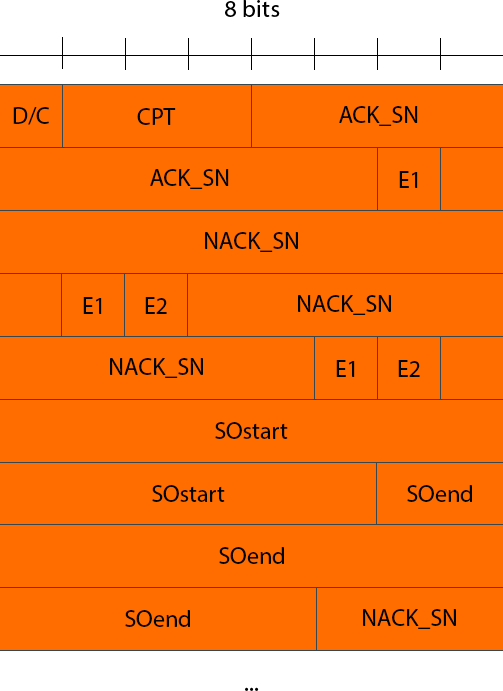
\includegraphics[width=0.4\textwidth]{images/rlc_status_pdu.png}}
	\caption{Umiejscowienie podwarstwy RLC w stosie protokołów LTE}
	\label{fig:status_pdu}
\end{figure}

Aby została ona wysłana musi zajść jedna z dwóch sytuacji:
\begin{enumerate}
	\item Licznik czasowy T status prohibit zakonczył odliczanie i została odebrana jednostka danych z włączoną flagą poll bit
	\item Liczniki czasowe T status prohibit i T reordering zakończyły odliczanie
\end{enumerate}

Licznik czasowy T status prohibit zapewnia, że ten sam pakiet status PDU nie zostanie wysłany kilkakrotnie. Jego odliczanie jest wznawiane po każdym wysłaniu pakietu status PDU.

Licznik czasowy T reordering jest startowany wówczas, gdy zostaną zauważone brakujące pakiety tj. gdy zostanie odebrany pakiet o numerze sekwencyjnym N a nie został jeszcze odebrany pakiet o numerze sekwencyjnym N - 1.

Flaga poll bit jest ustawiana po stronie nadajnika w następujących sytuacjach:
\begin{enumerate}
	\item Jeżeli pakietów wysłanych od czasu ostatniego potwierdzenia przekroczyła liczbę określoną przez parametr Poll PDU
	\item Jeżeli liczba bajtów wysłanych do odbiornika od czasu ostatniego potwierdzenia przekroczyła liczbę określoną przez parametr Poll Byte
	\item Jeżeli licznik czasowy T poll retransmit zakończył odliczanie i nie ma żadnych pakietów w buforze transmisji lub retransmisji (wówczas ponownie wysyłany jest ostatnio wysłany pakiet danych z ustawioną flagą poll bit)
\end{enumerate}


